\documentclass[11pt, a4paper]{MATH2023}
\usepackage{fancyhdr}
\usepackage{setspace}
\usepackage{amsmath,mathrsfs}
\usepackage{multicol}
\usepackage{amssymb}
\usepackage{graphicx}
\usepackage{caption}
\usepackage{subcaption}
\usepackage{xcolor}
\usepackage{enumitem}
\usepackage{tikz}
\usepackage{mathtools}
\usetikzlibrary{matrix}
\usepackage[normalem]{ulem}
\usepackage{multirow}
\usepackage[linesnumbered, ruled, boxed]{algorithm2e}
\SetKwRepeat{Do}{do}{while}
\newcommand{\eg}{\textbf{[Example.] }}
\newcommand{\sol}{\textbf{[Solution.] }}
\newcommand{\ii}{{\bf i}}
\newcommand{\jj}{{\bf j}}
\newcommand{\kk}{{\bf k}}
\newcommand{\rr}{{\bf r}}
\newcommand{\FF}{{\bf F}}
\newcommand{\nm}{\widehat{\bf n}}
\renewcommand{\div}{{\rm div\ }}
\newcommand{\curl}{{\rm curl\ }}
\newcommand{\pt}{\partial}


\title{Chapter 16}
\subtitle{Vector Calculus}

\begin{document}
\begin{spacing}{1.3}

    \section{The Divergence Theorem}


    \vspace{0.3in}
    {\it Since exam will not cover the proof, I'd like to omit here.}



    \newpage
    \section{Green's Theorem}
    \subsection{Green's Theorem in Line Integral}

    {\blue Recall what we have talked about in line integral: 
    \begin{enumerate}
        \item Arc length, 
        \item Mass:
    \end{enumerate}
    }

    Now consider doing line integral in a smooth simple {\bf closed curve} $C$ in the $xy$-plane,
    if $\FF(\rr)=P(\rr)\ii+Q(\rr)\jj$, then if we want to evaluate $\disp \oint_C\FF\cdot d\rr$,
    \begin{center}
        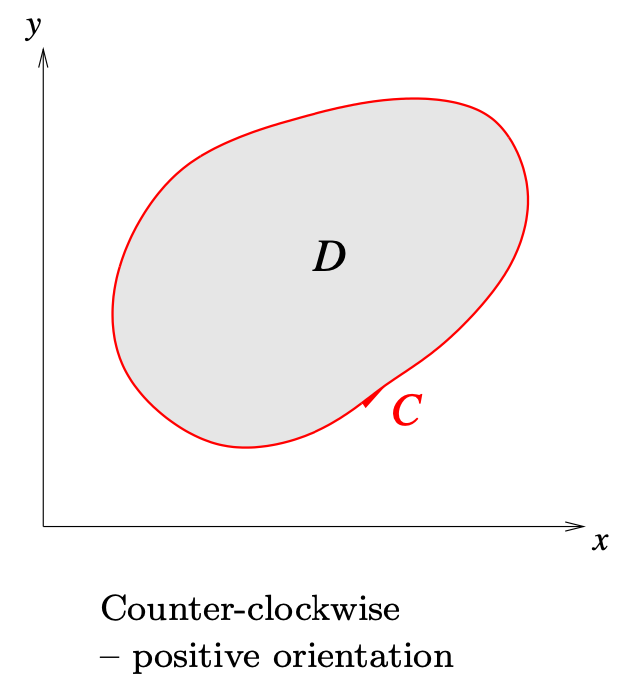
\includegraphics[scale=0.43]{images/Ch16-green-closed-path.png}
    \end{center}
    \begin{itemize}
        \item If $\FF$ is conservative, then line integral is 0, obviously.
        \item If $\FF$ is not conservative, then {\bf Green's Theorem} tells us 
        \begin{center}
            \boxed{$$\disp \oint_C \FF\cdot d\rr=\iint_D (\nabla \times \FF)\cdot \kk\ dA$$}
        \end{center}
    \end{itemize}
    {\bf Note} $\kk$ is the {\bf normal} to $xy$-plane, or, normal to region $D$.

    \vspace{0.3in}
    {\it Since exam will not cover the proof, I'd like to omit here.}

    
    
    
    \newpage
    {\blue This example shows how Green's Theorem simplify computation.}

    \eg $\disp \int_{C} x y d x+2 x^{2} d y$, $C$ consists of the segment from $(-2,0)$ to $(2,0)$ and top half of the circle
    $x^2+y^2=4$.
    \begin{center}
        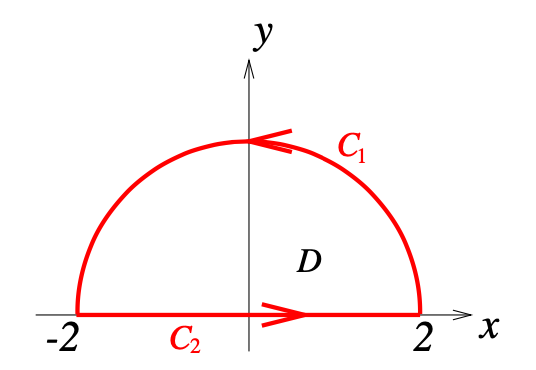
\includegraphics[scale=0.45]{images/Ch16-ex4.2.png}
    \end{center}
    
    \sol 
    
    {\bf Method 1:} use line integral: 
    $$ \int_{C} x y d x+2 x^{2} d y=\int_{C_{1}} x y d x+2 x^{2} d y+\int_{C_{2}} x y d x+2 x^{2} d y$$
    Parametrize the two curves:
    \begin{align*}
        C_{1} &: \mathbf{r}(t)=(1-t)(-2,0)+t(2,0)=(4 t-2,0) \quad 0 \leqslant t \leqslant 1 \\
        C_{2} &: \mathbf{r}(t)=(2 \cos t, 2 \sin t) \quad 0 \leqslant t \leqslant \pi
    \end{align*}
    Then directly evaluate the two line integrals
    \begin{align*}
        \int_{C_{1}} x y d x+2 x^{2} d y &=\int_{0}^{1}(4 t-2) \cdot 0 \cdot 4 d t+2(4 t-2)^{2} \cdot(0)=0 \\
        \int_{C_{2}} x y d x+2 x^{2} d y &=\int_{0}^{\pi}(2 \cos t)(2 \sin t)(-2 \sin t) d t+2(2 \cos t)^{2}(2 \cos t) d t \\
        &=8 \int_{0}^{\pi}\left(-\cos t \sin ^{2} t+\cos ^{3} t\right) d t=0
    \end{align*}
    Thus $\disp \int_{C} x y d x+2 x^{2} d y=0$.
    
    \vspace{0.5in}
    {\bf Method 2: } using Green's theorem:

    $\FF=(xy, 2x^2)$, hence $\nabla \times \FF=(4x-x)\kk =3x\kk$, then
    \begin{align*}
        \oint_{C} x y d x+2 x^{2} d y = \iint_D 3x dA &=\int_0^2\int_0^{\pi} 3r\cos\theta \ rd\theta dr \\
            &= \left. \int_0^2 3r^2\sin\theta \right|_0^{\pi} dr=0
    \end{align*}
    Actually, one may observe that $\disp \iint_D 3x dA=0$ directly, since $3x$ is a {\it odd} function in 
    $x$, and the region $D$ is {\it symmetric with respect to }$y$-axis.



    \newpage
    \subsection{Green's Theorem for computing Area}

    Recall that Green's Theorem states that:
    $$\oint_C \FF\cdot d\rr=\iint_D (\nabla \times \FF)\cdot \kk\ dA$$
    Notice if $\FF(\rr)=P(\rr)\ii+Q(\rr)\jj$,
    $$\oint_{C} \mathbf{F} \cdot d \mathbf{r}=\oint_{C} P d x+Q d y
    =\iint_{D}\left(\frac{\partial Q}{\partial x}-\frac{\partial P}{\partial y}\right) d A
    =\iint_D (\nabla \times \FF)\cdot \kk\ dA$$

    When $\disp \frac{\pt Q}{\pt x}-\frac{\pt P}{\pt y}=1$, then 
    \begin{center}
        \boxed{$$\disp A=\iint_D dA=\oint_C Pdx+Qdy$$.}
    \end{center}

    For example, when $P=0, Q=x$, or when $P=-y, Q=0$, or when $P=-y/2, Q=x/2$,
    $$A=\oint_C xdy=-\oint_C ydx=\frac{1}{2}\oint_C xdy-ydx$$



    \newpage
    {\blue The two examples below shows how to use Green's Theorem to find area.}

    \eg Find the area of $\disp \frac{x^2}{a^2}+\frac{y^2}{b^2}=1.$

    \sol Firstly parametrize the curve, let $x=a\cos\theta,\ y=b\sin\theta,\ 0\le \theta\le 2\pi$, then 
    $$C:\ \rr(\theta)=(a\cos\theta, b\sin\theta),\ 0\le \theta\le 2\pi$$,
    If we choose $\disp \FF(\rr)=P(\rr)\ii+Q(\rr)\jj=-\frac{y}{2}\ii+\frac{x}{2}\jj$, then we have
    $$\frac{\pt Q}{\pt x}-\frac{\pt P}{\pt y}=\frac{1}{2}+\frac{1}{2}=1$$
    Hence, 
    \begin{align*}
        D &= \frac{1}{2} \oint (xdy-ydx)\\
        &= \frac{1}{2} \left[ \int_0^{2\pi} a\cos\theta\cdot b\cos\theta\ d\theta 
        + b\sin\theta\cdot a\sin\theta\ d\theta \right]\\
        &= \frac{1}{2} ab \cdot \int_0^{2\pi} (\cos^2\theta+\sin^2\theta)\ d\theta =\pi ab
    \end{align*}


    \vspace{\fill}
    \eg Find the area of the hypocycloid $x^{2 / 3}+y^{2 / 3}=a^{2 / 3}$.
    \begin{center}
        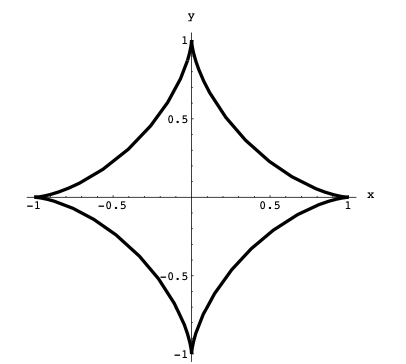
\includegraphics[scale=0.55]{images/Ch16-green-area-eg2.png}
    \end{center}

    \sol 
    Firstly parametrize the curve, 
    let $x=a \cos ^{3} \theta, y=a \sin ^{3} \theta, \quad$ where $0 \leqslant \theta \leqslant 2 \pi$,

    Again, use vector field $\disp \FF(\rr)=P(\rr)\ii+Q(\rr)\jj=-\frac{y}{2}\ii+\frac{x}{2}\jj$,
    \begin{align*}
        A=\frac{1}{2} \oint_{C} x d y-y d x &=\frac{1}{2} \int_{0}^{2 \pi}\left(a \cos ^{3} \theta \times 3 a \sin ^{2} \theta \cos \theta d \theta+a \sin ^{3} \theta \times 3 a \cos ^{2} \theta \sin \theta d \theta\right) \\
        &=\frac{3}{2} a^{2} \int_{0}^{2 \pi}\left(\cos ^{4} \sin ^{2} \theta+\sin ^{4} \theta \cos ^{2} \theta\right) d \theta \\
        &=\frac{3}{2} a^{2} \int_{0}^{2 \pi} \frac{1}{4} \sin ^{2} 2 \theta d \theta \\
        &=\frac{3}{8} a^{2} \int_{0}^{2 \pi}\left(\frac{1-\cos 4 \theta}{2}\right) d \theta=\frac{3 \pi}{8} a^{2}
    \end{align*}



    \newpage
    \subsection{General version of Green’s Theorem}

    {\blue {\it This part will not be covered in exam.}}

    Recall that Green's Theorem only applies to {\it simple} and {\it closed} curve. 
    However, it can be extended to apply to region with holes. We simply cut the region 
    into some regions that without holes, for example:
    \begin{center}
        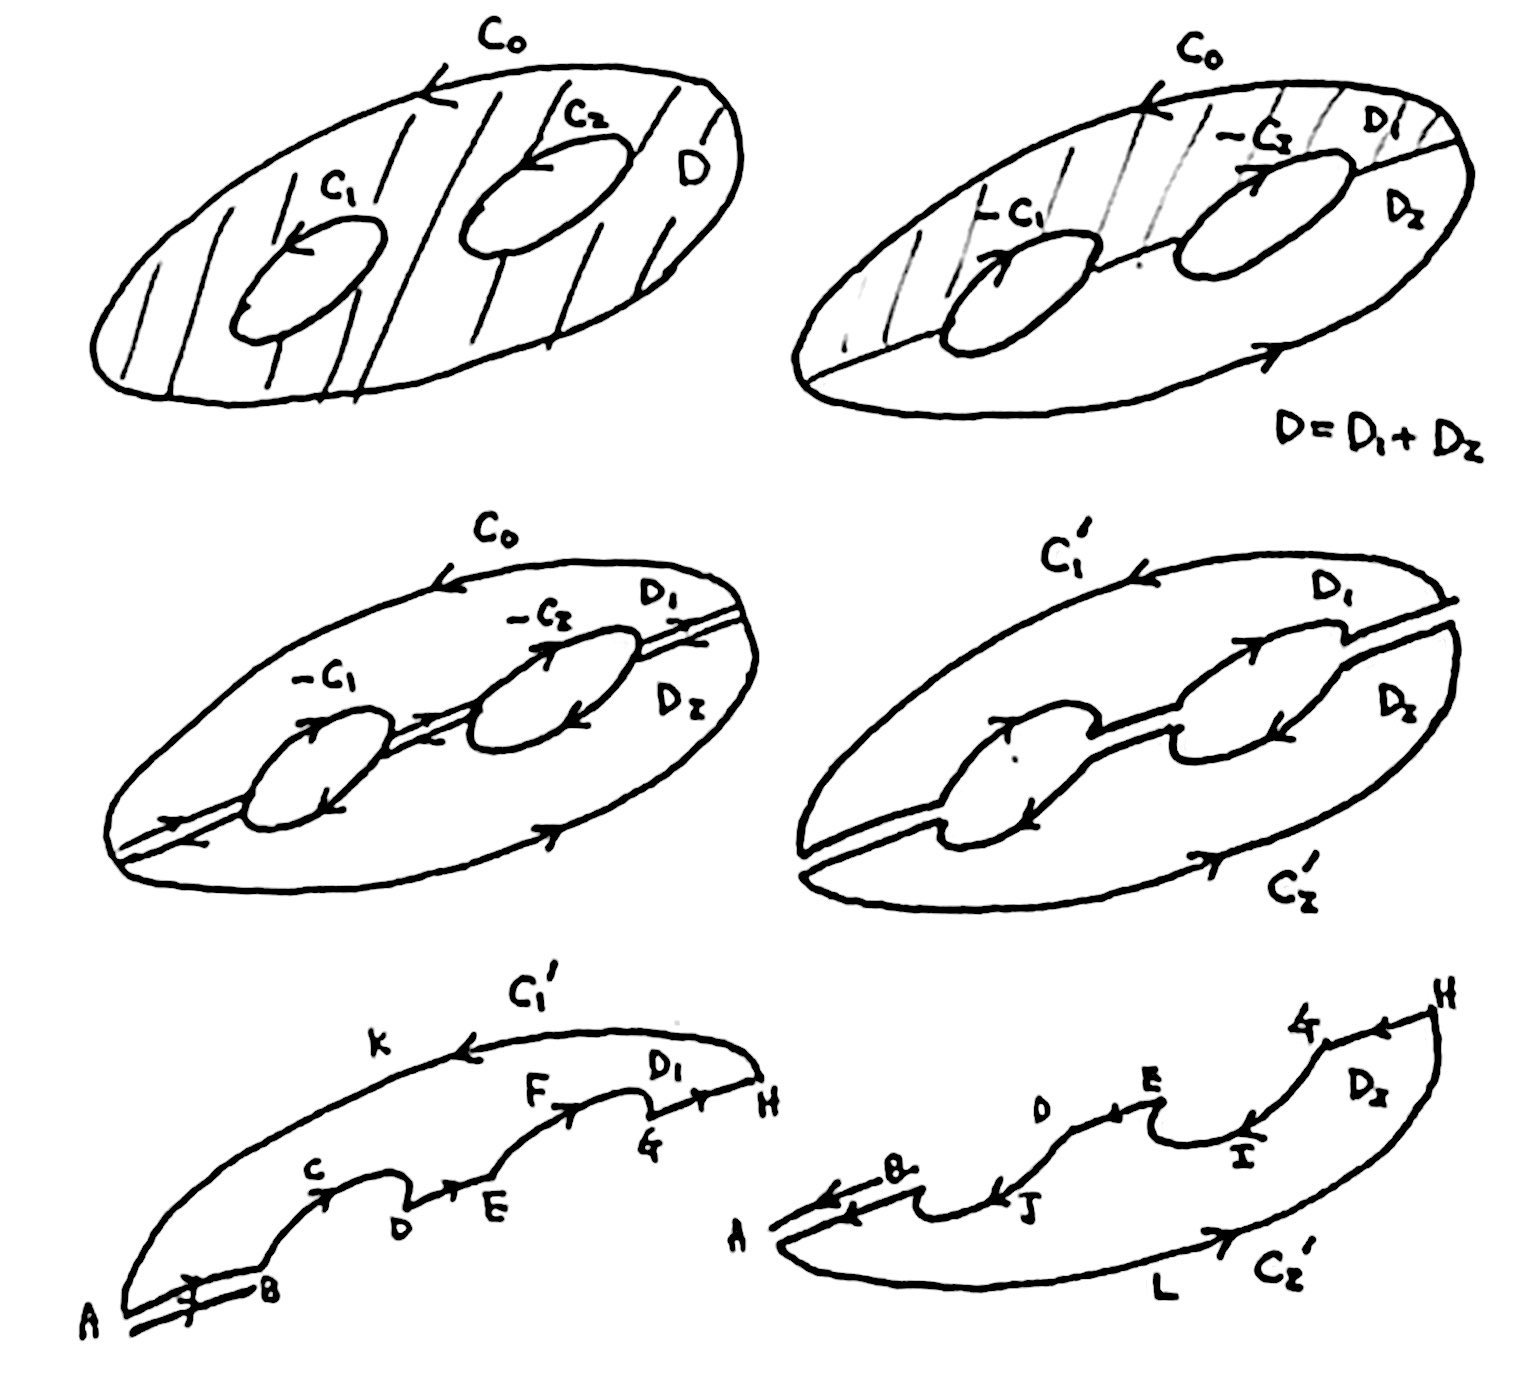
\includegraphics[scale=0.23]{images/Ch16-general-green.JPG}
    \end{center}
    \begin{align*}
        \iint_D &= \iint_{D_1}+\iint_{D_2} = \oint_{C_1^\prime}+\oint_{C_2^\prime}\\
        &= \left( \int_{HKA}+\int_{AB}+\int_{BCD}+\int_{DE}+\int_{EFG}+\int_{GH} \right)
        + \left( \int_{ALH}+\int_{HG}+\int_{GIE}+\int_{ED}+\int_{DJB}+\int_{BA} \right)\\
        &= \int_{C_0}-\int_{C_1}-\int_{C_2}
    \end{align*}



    \newpage
    {\blue Here is the example provided in lecture note.}
    
    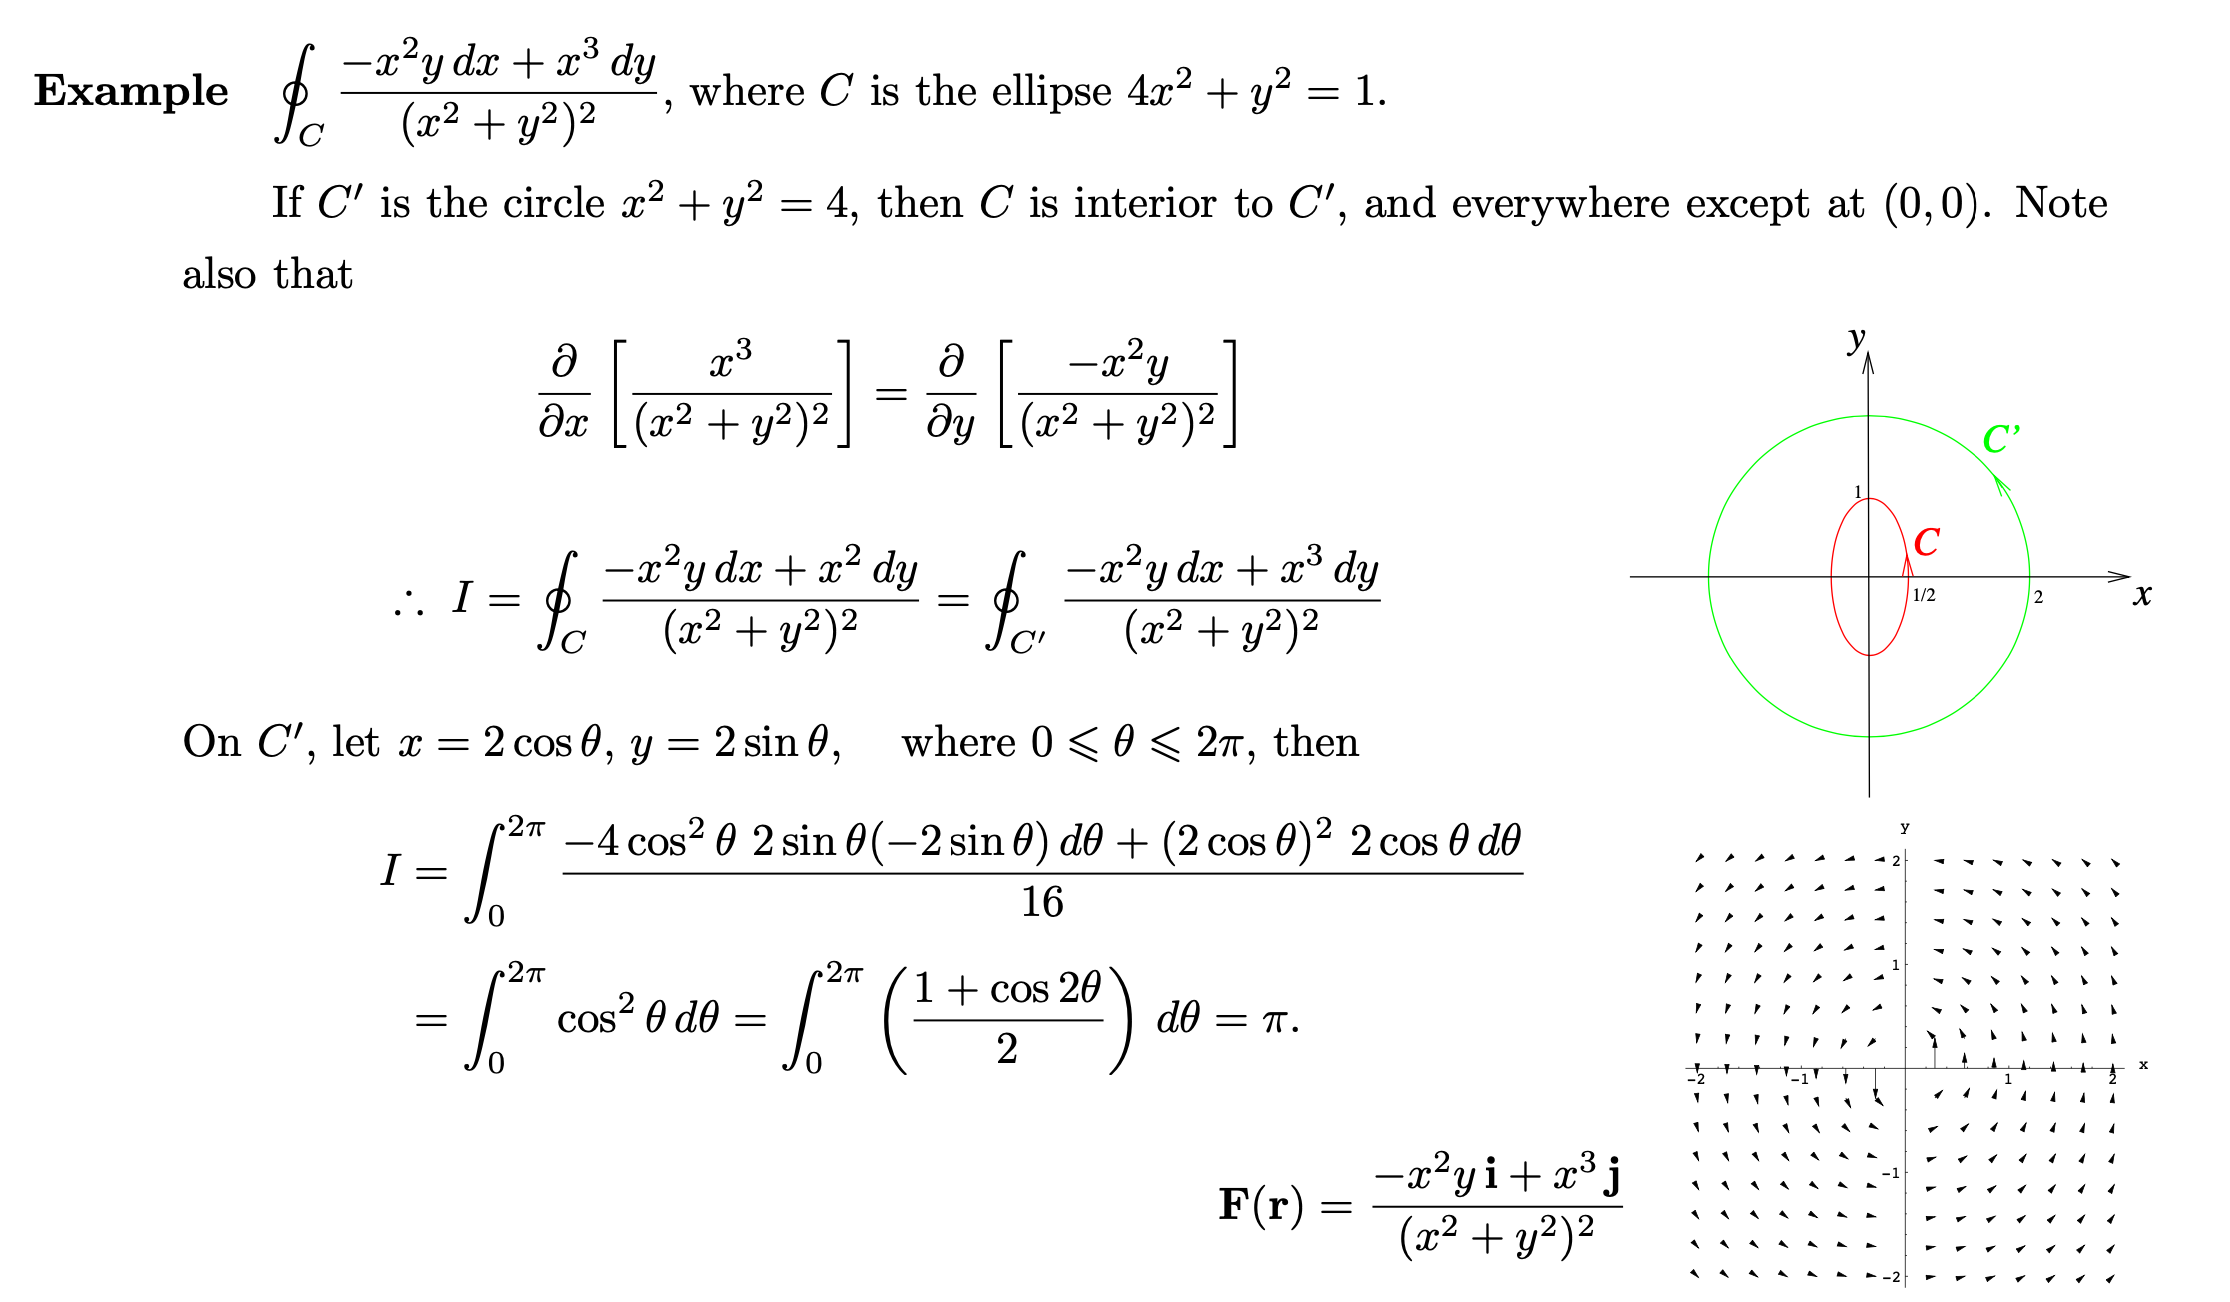
\includegraphics[scale=0.44]{images/Ch16-general-green-eg.png}



    \newpage
    \section{Stokes’ Theorem}



    \vspace{\fill}
    \begin{center}
        {\it This is the end of Chapter 16, and the end of this course!}
    \end{center}

    

\end{spacing}
\end{document}
